\chapter{Procesado de la imagen de color}
\label{chap:Procesado de la imagen de color}
\Abstract{El presente capítulo describe de forma detallada el trabajo realizado en cuanto al procesamiento de imágenes de color. Para ello se repasan los procedimientos empleados en las imágenes de color y se muestran los resultados de estos procedimientos.}

El primer paso para poder recolocar piezas es localizarlas. Con el objetivo de localizarlas, se han desarrollado múltiples herramientas capaces de hacerlo, pero cada una presenta grandes ventajas y desventajas. Pero para poder entender la evolución y el desarrollo de estas es necesario entender el contexto de este proyecto. Se parte del trabajo previo llevado acabo por Ana Berjón \cite{TFGAna}, y el objetivo de este proyecto era el perfeccionamiento de este sistema. Tanto el perfeccionamiento del procesado de la imagen como de la interacción con el robot. Desgraciadamente, debido a una pandemia ha sido imposible poder trabajar con el brazo robótico y por ello este proyecto se ha centrado solo en el procesado de la imagen.

Teniendo todo lo anterior en cuenta, se puede entender la evolución del proyecto:
\begin{itemize}
\item Perfeccionamiento del sistema basado en filtros de color, detección de borde y de formas.
\item Desarrollo de clasificadores
\item Desarrollo de detectores basados en los clasificadores y R-CNN.
\item Desarrollo de detectores basados en los clasificadores y Faster R-CNN.
\item Desarrollo de detectores basados en los clasificadores y YOLO.
\end{itemize}
A continuación, se van a desarrollar de forma individual cada uno de estos métodos explicando su estructura, funcionamiento y capacidades. Por último, se hará una comparativa de todos los métodos desarrollados.

\section{Colour analysis}
\label{sec:Colour analysis}
Como su nombre indica, es un proceso que depende fuertemente del filtrado de color. Esto se debe a que para localizar las piezas, obtener sus características y su orientación es recomendable trabajar en escala de grises e imágenes binarias. Pero para esta aplicación también es necesario saber el color de la pieza. Por ello primero se debe de filtrar por color para poder separar las piezas. Esta etapa es crucial y por ello también es el motivo de fallo del sistema. Como se verá mas adelante, cambios en la iluminación pueden implicar un fallo catastrófico y el sistema deja de ser capaz de identificar piezas.

Para analizar cada imagen, se debe de repetir el mismo proceso para cada posible color de las piezas de LEGO. Este proceso a seguir se puede dividir en tres etapas:

\subsection{Filtrado de color}
Se aplican tres filtros de color a la imagen original con el objetivo de separar las piezas y clasificar las por su color. Para trabajar con mayor facilidad y precisión, primero se transforma la imagen a el formato hsv. A continuación se crea la mascara binaria, para ello se comparan los pixeles de la imagen en formato hsv, frente a unos máximos y mínimos. Si el pixel se encuentra dentro de los valores permitidos, se representara en la imagen binaria como un uno, en caso contrario será un cero. De esta forma, se obtienen las mascaras mostradas en la columna del medio de la\autoref{fig:colour}. Y multiplicando la imagen original por la imagen binaria, se obtienen las imágenes de la última columna.

Desgraciadamente, cambios en la iluminación pueden modificar drásticamente los resultados de los filtros de color. Este proceso se puede ver a continuación en la \autoref{fig:colour2}. Para evitar que esto suceda, es recomendable calibrar de forma regular los filtros de color y asegurarse de que las condiciones lumínicas permanezcan lo mas constante posibles.

\begin{figure}[ht]  %Error filtro de color
  \subfloat{
	\begin{minipage}[c][1\width]{0.3\textwidth}
	   \centering
	   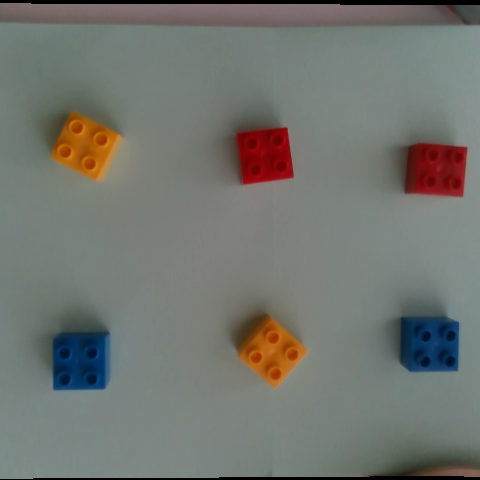
\includegraphics[width=1\textwidth]{Procesado de la imagen de color/Colour Analysis/colour.png}
	\end{minipage}}
  \hfill	
  \subfloat{
	\begin{minipage}[c][1\width]{0.3\textwidth}
	   \centering
	   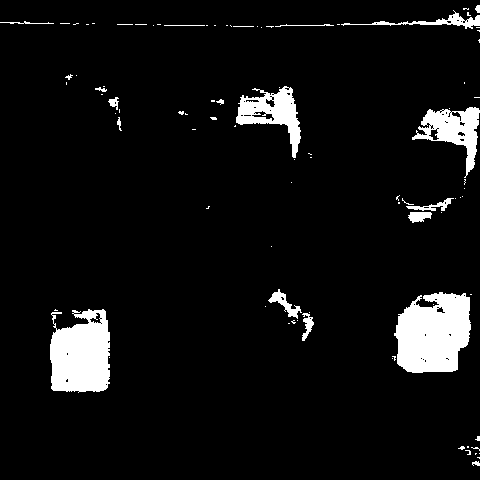
\includegraphics[width=1\textwidth]{Procesado de la imagen de color/Colour Analysis/error_binario.png}
	\end{minipage}}
  \hfill	
  \subfloat{
	\begin{minipage}[c][1\width]{0.3\textwidth}
	   \centering
	   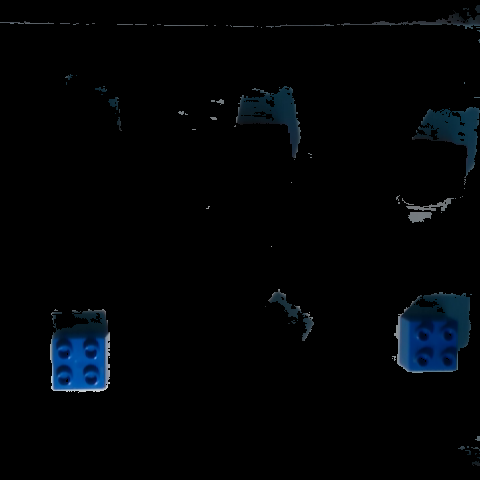
\includegraphics[width=1\textwidth]{Procesado de la imagen de color/Colour Analysis/error.png}
	\end{minipage}}
\caption{Error por mala calibración del filtrado por color}
\label{fig:colour2}
\vspace{-5pt}
\end{figure}

Para el desarrollo de los filtros por color, se ha usado una herramienta de MATLAB llamada colorThresholder. Con la ayuda de esta herramienta se han creado tres funciones. Una función para cada color la cual devuelve la imagen binaria y la combinación de la imagen original y la imagen binaria.

\begin{figure}[ht]  %Filtrado por color
  \subfloat{
	\begin{minipage}[c][1\width]{0.3\textwidth}
	   \centering
	   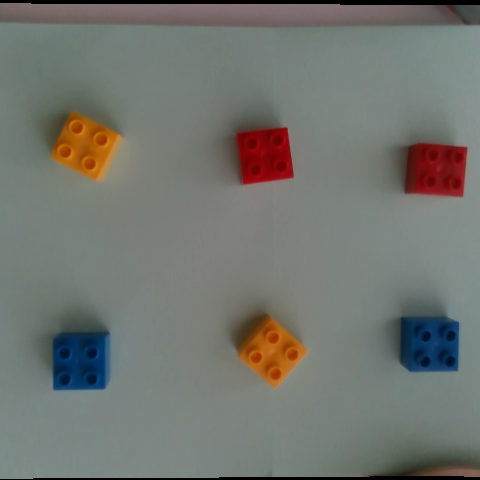
\includegraphics[width=1\textwidth]{Procesado de la imagen de color/Colour Analysis/colour.png}
	\end{minipage}}
  \hfill	
  \subfloat{
	\begin{minipage}[c][1\width]{0.3\textwidth}
	   \centering
	   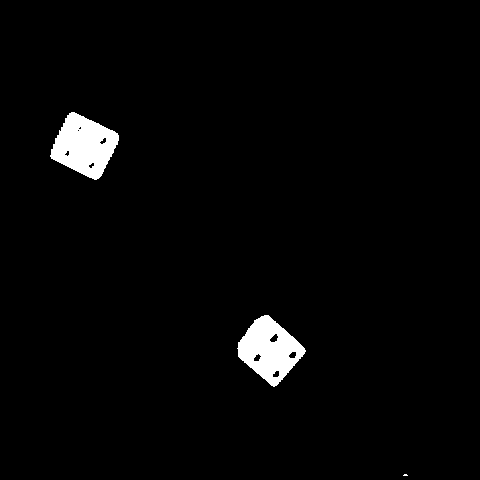
\includegraphics[width=1\textwidth]{Procesado de la imagen de color/Colour Analysis/yellow_binario.png}
	\end{minipage}}
  \hfill	
  \subfloat{
	\begin{minipage}[c][1\width]{0.3\textwidth}
	   \centering
	   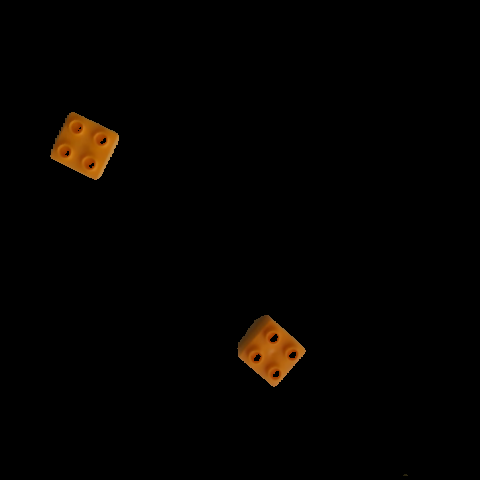
\includegraphics[width=1\textwidth]{Procesado de la imagen de color/Colour Analysis/yellow.png}
	\end{minipage}}
  
  \medskip
  
  \subfloat{
	\begin{minipage}[c][1\width]{0.3\textwidth}
	   \centering
	   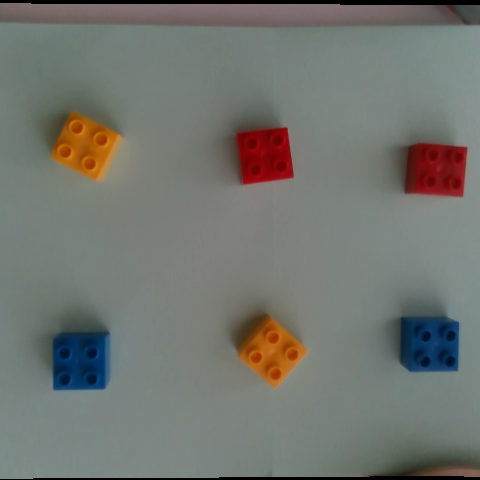
\includegraphics[width=1\textwidth]{Procesado de la imagen de color/Colour Analysis/colour.png}
	\end{minipage}}
  \hfill	
  \subfloat{
	\begin{minipage}[c][1\width]{0.3\textwidth}
	   \centering
	   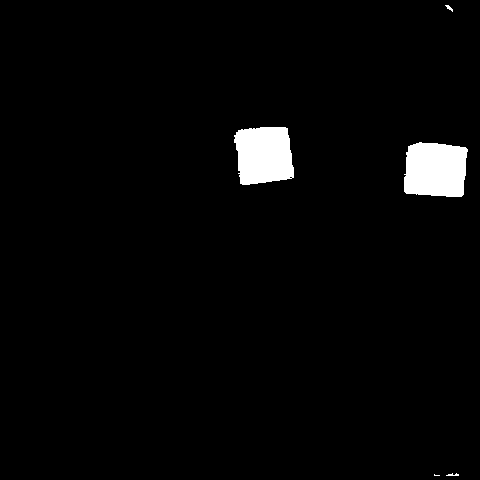
\includegraphics[width=1\textwidth]{Procesado de la imagen de color/Colour Analysis/red_binario.png}
	\end{minipage}}
  \hfill	
  \subfloat{
	\begin{minipage}[c][1\width]{0.3\textwidth}
	   \centering
	   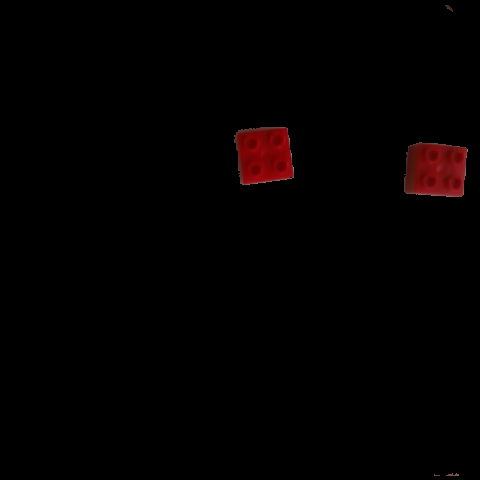
\includegraphics[width=1\textwidth]{Procesado de la imagen de color/Colour Analysis/red.png}
	\end{minipage}}
	
  \medskip
  
  \subfloat{
	\begin{minipage}[c][1\width]{0.3\textwidth}
	   \centering
	   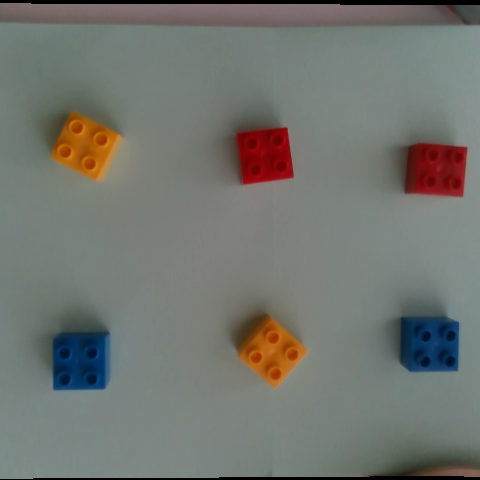
\includegraphics[width=1\textwidth]{Procesado de la imagen de color/Colour Analysis/colour.png}
	\end{minipage}}
  \hfill	
  \subfloat{
	\begin{minipage}[c][1\width]{0.3\textwidth}
	   \centering
	   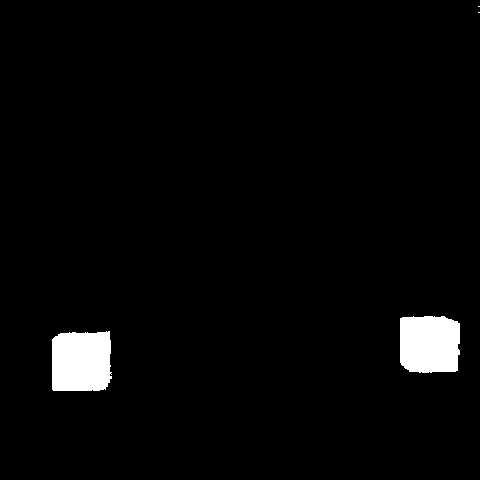
\includegraphics[width=1\textwidth]{Procesado de la imagen de color/Colour Analysis/blue_binario.png}
	\end{minipage}}
  \hfill	
  \subfloat{
	\begin{minipage}[c][1\width]{0.3\textwidth}
	   \centering
	   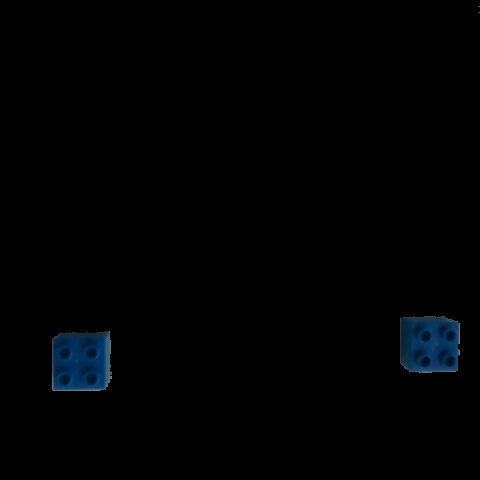
\includegraphics[width=1\textwidth]{Procesado de la imagen de color/Colour Analysis/blue.png}
	\end{minipage}}
\caption{Filtrado por color}
\label{fig:colour}
\end{figure}

\clearpage
\subsection{Identificación y mejora de la imagen}
Una vez aplicado el filtro de color se realiza un estudio exhaustivo de las piezas. Este comienza por la separación de la piezas para cada color. Para ello, primero se hace una limpieza de la imagen eliminando los pequeños objetos de la imagen binaria (ruido). A continuación, se emplea la función de MATLAB regionprops que devuelve las propiedades de los objetos encontrados y el número de objetos encontrados. De esta forma, ya sabemos el número de piezas de cada color y de forma aproximada su posición y área.

Desgraciadamente la información extraída con regionprops no es suficientemente precisa. Sobretodo cuando se tienen varias piezas apiladas ya que con los filtros también se puede haber detectado las piezas inferiores aumentando así el tamaño de la pieza. Por ello es necesario un estudio más exhaustivo analizando cada pieza de forma independiente. Para facilitar el calculo y la mejor detección de la pieza, se pasan todas las piezas a escala de grises \citep{greyscale}. A continuación se muestran el proceso de separación de piezas y transformación a escala de grises.

\begin{figure}[ht]  %Selección de la pieza
  \subfloat{
	\begin{minipage}[c][1\width]{0.3\textwidth}
	   \centering
	   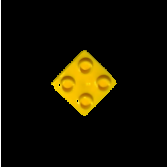
\includegraphics[width=1\textwidth]{Procesado de la imagen de color/Colour Analysis/amarillo_aux.png}
	\end{minipage}}
  \hfill	
  \subfloat{
	\begin{minipage}[c][1\width]{0.3\textwidth}
	   \centering
	   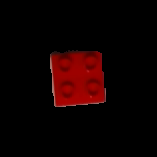
\includegraphics[width=1\textwidth]{Procesado de la imagen de color/Colour Analysis/red_aux.png}
	\end{minipage}}
  \hfill	
  \subfloat{
	\begin{minipage}[c][1\width]{0.3\textwidth}
	   \centering
	   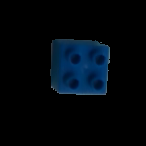
\includegraphics[width=1\textwidth]{Procesado de la imagen de color/Colour Analysis/blue_aux.png}
	\end{minipage}}
\caption{Selección de la pieza a analizar}
\label{fig:mejora1}
\vspace{-5pt}
\end{figure}

\begin{figure}[ht]  %Escalado de grises
  \subfloat{
	\begin{minipage}[c][1\width]{0.3\textwidth}
	   \centering
	   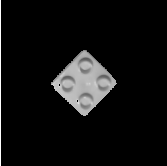
\includegraphics[width=1\textwidth]{Procesado de la imagen de color/Colour Analysis/amarillo_aux_ad.png}
	\end{minipage}}
  \hfill	
  \subfloat{
	\begin{minipage}[c][1\width]{0.3\textwidth}
	   \centering
	   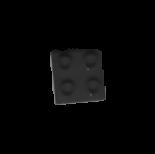
\includegraphics[width=1\textwidth]{Procesado de la imagen de color/Colour Analysis/red_aux_ad.png}
	\end{minipage}}
  \hfill	
  \subfloat{
	\begin{minipage}[c][1\width]{0.3\textwidth}
	   \centering
	   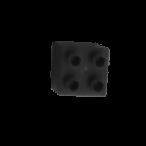
\includegraphics[width=1\textwidth]{Procesado de la imagen de color/Colour Analysis/blue_aux_ad.png}
	\end{minipage}}
\caption{Escalado de grises}
\label{fig:mejora2}
\vspace{-5pt}
\end{figure}

El proceso a seguir para mejorar la precisión de la detección de la pieza consiste en eliminar el borde de la pieza y los elementos pequeños. De esta forma se intenta solo detectar la cara superior del LEGO. Una vez eliminado el borde se vuelve a emplear regionprops para obtener todas las propiedades pero con una mayor precisión.

Para poder detectar correctamente el borde y eliminarlo de la imagen primero es necesario ajustar y filtrar la imagen. El proceso total de mejora de la imagen y extracción de características consta de ocho pasos:

\begin{itemize}
\item Primer paso: ajuste de de la intensidad de la imagen en escala de grises. De esta forma se resaltan más los cambios de color/iluminación.

\item Segundo y tercer paso: se desea resaltar aun más los detalles de la imagen. Esto se va a llevar a cabo con la ayuda de un filtro de difuminado Gaussiano. Primero se difumina la imagen para ensalzar las rasgos generales y después se le restan estos rasgos a la imagen original. De esta forma se destacan las pequeños detalles.

\item Cuarto paso: Una vez mejorada la imagen, toca detectar el borde de la pieza. Para ello se va a aplicar el algoritmo de Canny.

\item Quinto paso: Al filtrar las imágenes por color también se puede haber incluido las caras laterales de la pieza y las caras laterales de las piezas situadas debajo de la pieza a detectar. Para reducir el efecto que esto puede causar, se ensanchan los bordes de forma que incluyan pequeños detalles que puedan estropear el proceso.

\item Sexto paso: el último paso para obtener la cara interna del LEGO consiste en invertir los colores de los bordes obtenidos. De esta forma, solo se conserva la cara interna.
\end{itemize}

\begin{figure}[ht!]  %Primer paso
  \subfloat{
	\begin{minipage}[c][1\width]{0.3\textwidth}
	   \centering
	   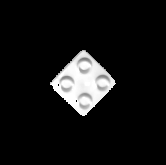
\includegraphics[width=1\textwidth]{Procesado de la imagen de color/Colour Analysis/amarillo_ad.png}
	\end{minipage}}
  \hfill	
  \subfloat{
	\begin{minipage}[c][1\width]{0.3\textwidth}
	   \centering
	   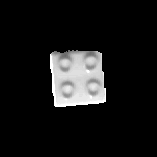
\includegraphics[width=1\textwidth]{Procesado de la imagen de color/Colour Analysis/red_ad.png}
	\end{minipage}}
  \hfill	
  \subfloat{
	\begin{minipage}[c][1\width]{0.3\textwidth}
	   \centering
	   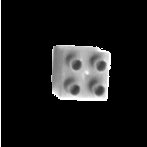
\includegraphics[width=1\textwidth]{Procesado de la imagen de color/Colour Analysis/blue_ad.png}
	\end{minipage}}
\caption{Primer paso: ajuste de intensidad}
\label{fig:mejora3}
\vspace{-5pt}
\end{figure}

\begin{figure}[ht!]  %Segundo y tercer paso
  \subfloat{
	\begin{minipage}[c][1\width]{0.3\textwidth}
	   \centering
	   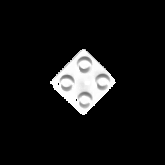
\includegraphics[width=1\textwidth]{Procesado de la imagen de color/Colour Analysis/amarillo_fin2.png}
	\end{minipage}}
  \hfill	
  \subfloat{
	\begin{minipage}[c][1\width]{0.3\textwidth}
	   \centering
	   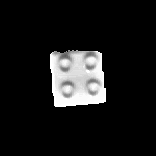
\includegraphics[width=1\textwidth]{Procesado de la imagen de color/Colour Analysis/red_fin2.png}
	\end{minipage}}
  \hfill	
  \subfloat{
	\begin{minipage}[c][1\width]{0.3\textwidth}
	   \centering
	   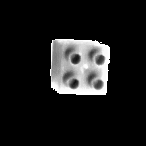
\includegraphics[width=1\textwidth]{Procesado de la imagen de color/Colour Analysis/blue_fin2.png}
	\end{minipage}}
\caption{Segundo y tercer paso: Resalto de pequeños detalles}
\label{fig:mejora4}
\vspace{-5pt}
\end{figure}

\begin{figure}[ht!]  %Cuarto paso
  \subfloat{
	\begin{minipage}[c][1\width]{0.3\textwidth}
	   \centering
	   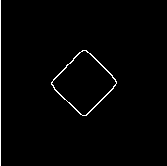
\includegraphics[width=1\textwidth]{Procesado de la imagen de color/Colour Analysis/amarillo_f.png}
	\end{minipage}}
  \hfill	
  \subfloat{
	\begin{minipage}[c][1\width]{0.3\textwidth}
	   \centering
	   
\includegraphics[width=1\textwidth]{Procesado de la imagen de color/Colour Analysis/red_f.png}
	\end{minipage}}
  \hfill	
  \subfloat{
	\begin{minipage}[c][1\width]{0.3\textwidth}
	   \centering
	   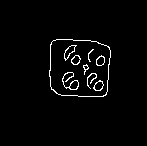
\includegraphics[width=1\textwidth]{Procesado de la imagen de color/Colour Analysis/blue_f.png}
	\end{minipage}}
\caption{Cuarto paso: aplicación del algoritmo de Canny}
\label{fig:mejora5}
\vspace{-5pt}
\end{figure}

\begin{figure}[ht!]	 %Quinto paso
  \subfloat{
	\begin{minipage}[c][1\width]{0.3\textwidth}
	   \centering
	   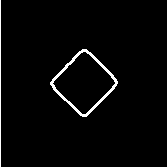
\includegraphics[width=1\textwidth]{Procesado de la imagen de color/Colour Analysis/amarillo_d.png}
	\end{minipage}}
  \hfill	
  \subfloat{
	\begin{minipage}[c][1\width]{0.3\textwidth}
	   \centering
	   
\includegraphics[width=1\textwidth]{Procesado de la imagen de color/Colour Analysis/red_c.png}
	\end{minipage}}
  \hfill	
  \subfloat{
	\begin{minipage}[c][1\width]{0.3\textwidth}
	   \centering
	   
\includegraphics[width=1\textwidth]{Procesado de la imagen de color/Colour Analysis/blue_c.png}
	\end{minipage}}
\caption{Quinto paso: dilatación y contracción de los bordes}
\label{fig:mejora6}
\vspace{-5pt}
\end{figure}

\begin{figure}[ht!]  %Sexto paso
  \subfloat{
	\begin{minipage}[c][1\width]{0.3\textwidth}
	   \centering
	   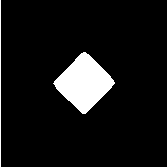
\includegraphics[width=1\textwidth]{Procesado de la imagen de color/Colour Analysis/amarillo_b.png}
	\end{minipage}}
  \hfill	
  \subfloat{
	\begin{minipage}[c][1\width]{0.3\textwidth}
	   \centering
	   
\includegraphics[width=1\textwidth]{Procesado de la imagen de color/Colour Analysis/red_b.png}
	\end{minipage}}
  \hfill	
  \subfloat{
	\begin{minipage}[c][1\width]{0.3\textwidth}
	   \centering
	   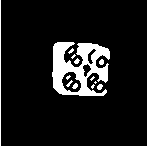
\includegraphics[width=1\textwidth]{Procesado de la imagen de color/Colour Analysis/blue_b.png}
	\end{minipage}}
\caption{Sexto paso: Inversión de los colores de la pieza}
\label{fig:mejora7}
\vspace{-5pt}
\end{figure}

\newpage
\subsection{Extracción de características}
El último paso para la obtención de las características de la pieza se vuelve a emplear la función regionprops de MATLAB. con cada una de las piezas identificadas. Al trabajarse de forma individual con cada pieza y como estan has sido mejoradas, la precisión es bastante elevada y se puede obtener de forma bastante precisa el centroide de cada pieza.

\subsection{Resultados}
Para comprobar la eficacia de Colour analysis, se ha desarrollado un script con la ayuda de MATLAB para determinar su capacidad de para identificar piezas y la precisión con las que la detecta. En este script se han analizado \rev{X imágenes} con más de \rev{X piezas de LEGO}.

Para poder realizar un análisis rigoroso y que refleje la capacidad de este método ante diversas condiciones, se han seleccionado fotos con múltiples ángulos y escenas. Y se han obtenido los siguientes resultados:

\begin{figure}[ht]  %Estudio Amarillo
  \subfloat{
	\begin{minipage}[c][1\width]{0.49\textwidth}
	   \centering
	   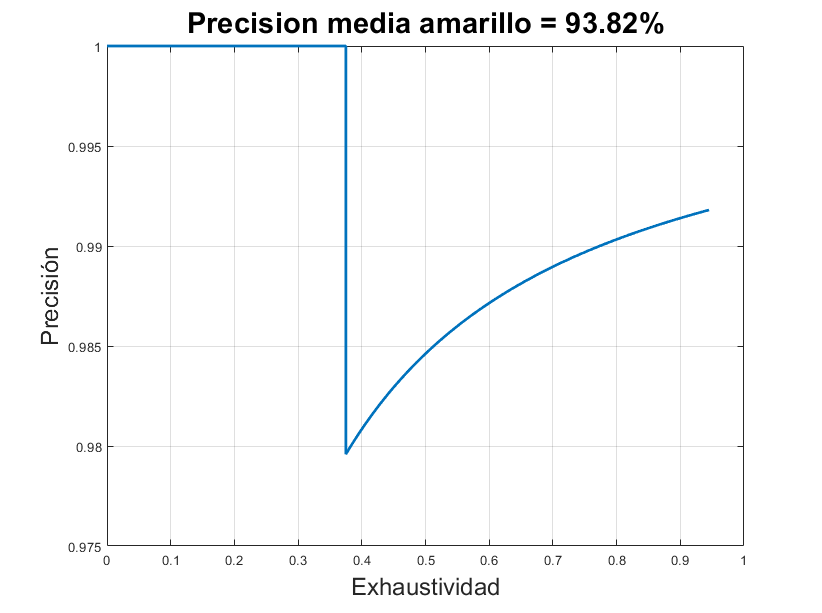
\includegraphics[width=1\textwidth]{Procesado de la imagen de color/Colour Analysis/precision_yellow.png}
	\end{minipage}}
  \hfill	
  \subfloat{
	\begin{minipage}[c][1\width]{0.49\textwidth}
	   \centering
	   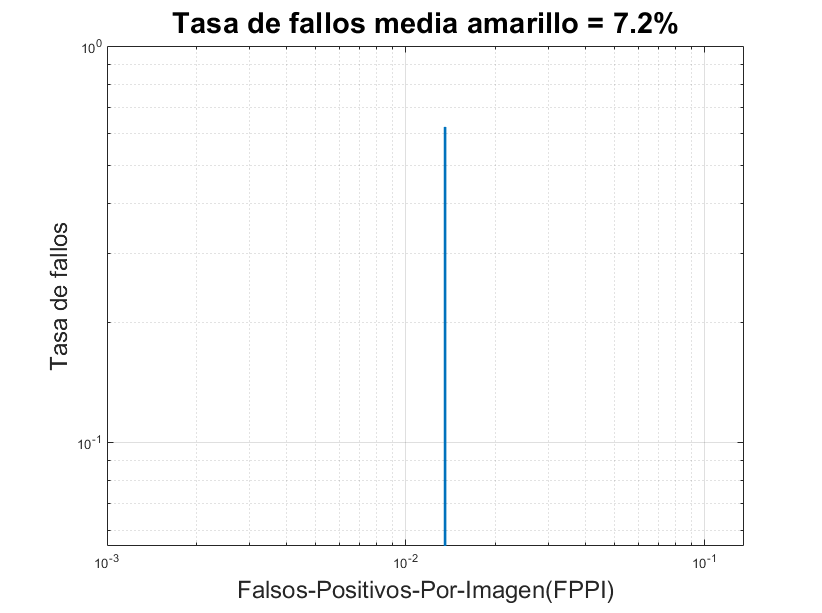
\includegraphics[width=1\textwidth]{Procesado de la imagen de color/Colour Analysis/miss_yellow.png}
	\end{minipage}}
\caption{Estudio de Colour analysis al detectar piezas amarillas}
\label{fig:yellow colour}
\vspace{-5pt}
\end{figure}

\begin{figure}[ht]  %Estudio Rojo
  \subfloat{
	\begin{minipage}[c][1\width]{0.49\textwidth}
	   \centering
	   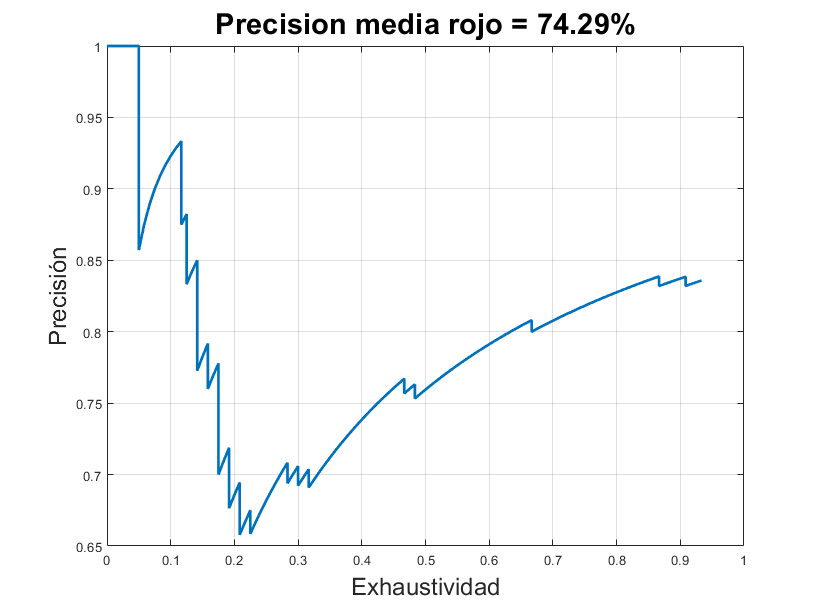
\includegraphics[width=1\textwidth]{Procesado de la imagen de color/Colour Analysis/precision_red.png}
	\end{minipage}}
  \hfill	
  \subfloat{
	\begin{minipage}[c][1\width]{0.49\textwidth}
	   \centering
	   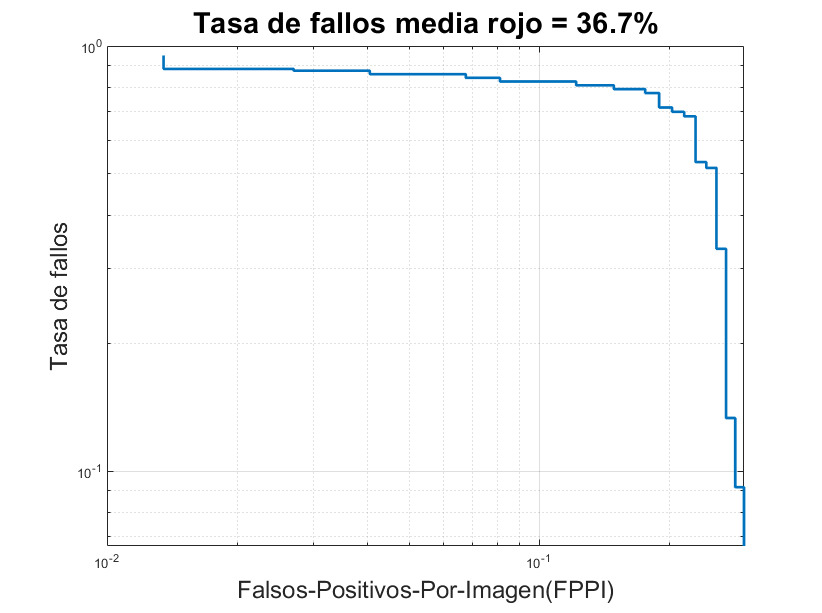
\includegraphics[width=1\textwidth]{Procesado de la imagen de color/Colour Analysis/miss_red.png}
	\end{minipage}}
\caption{Estudio de Colour analysis al detectar piezas rojas}
\label{fig:red colour}
\vspace{-5pt}
\end{figure}

\begin{figure}[ht]  %Estudio Azul
  \subfloat{
	\begin{minipage}[c][1\width]{0.49\textwidth}
	   \centering
	   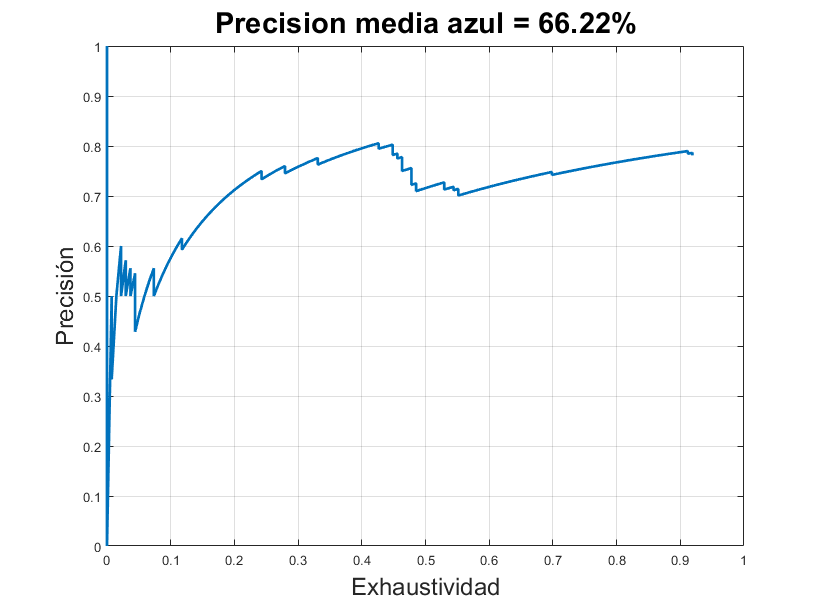
\includegraphics[width=1\textwidth]{Procesado de la imagen de color/Colour Analysis/precision_blue.png}
	\end{minipage}}
  \hfill	
  \subfloat{
	\begin{minipage}[c][1\width]{0.49\textwidth}
	   \centering
	   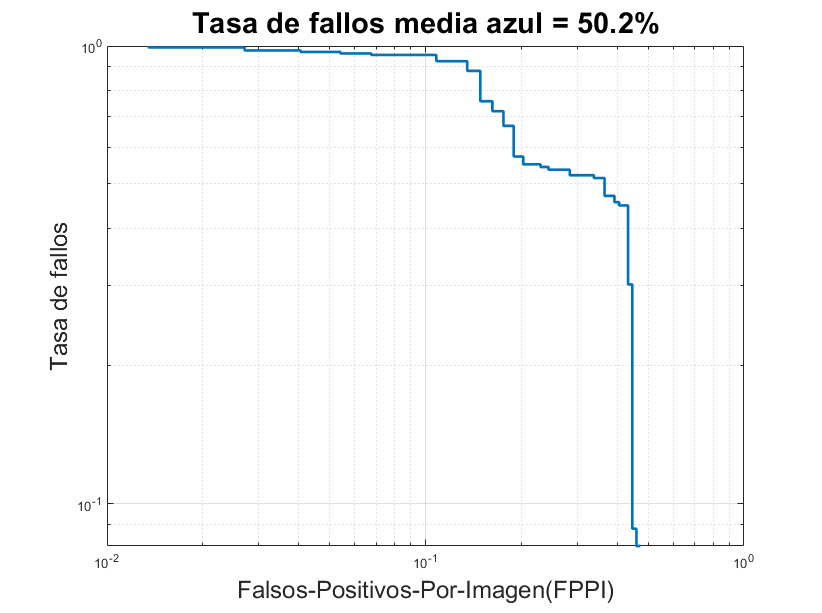
\includegraphics[width=1\textwidth]{Procesado de la imagen de color/Colour Analysis/miss_blue.png}
	\end{minipage}}
\caption{Estudio de Colour analysis al detectar piezas azules}
\label{fig:blue colour}
\vspace{-5pt}
\end{figure}

\newpage
\section{Clasificadores}
Los clasificadores son redes neuronales diseñadas con el objetivo de identificar. Estos no son capaces de localizar un objeto, sino que solo son capaces de indicar si el objeto está en la imagen o no. En este proyecto identificar los objetos no es suficiente ya que también hace falta localizarlos. A pesar de ello, primero se van a entrenar dos clasificadores con el objetivo de que sirvan como base para el desarrollo del los detectores de objetos.

Por falta tanto de datos como de cálculo computacional, se va a partir de dos clasificadores ya entrenados y se van a reentrenar. De esta forma podemos partir de dos clasificadores con estructuras ampliamente corroboradas a la vez que se consigue reducir la carga computacional y con ello el tiempo de entrenamiento.

Los dos clasificadores elegidos para ser reentrenados son AlexNet y VGG-16. Los motivos de su elección son: Se caracterizan por redes simples y lineales lo cual facilita su comprensión y el trabajo con ellas. Reflejan la evolución de las redes neuronales durante los últimos años. Los dos nuevos clasificadores han sido nombrados como LEGONet y LEGO16 respectivamente. De ahora en adelante se referirá a ellos de esta forma.

\subsection{LEGONet}
Originalmente AlexNet fue diseñado para trabajar con la base de datos de ImageNet, que cuenta con más de 14 millones de fotos y 1000 clases diferentes. Para este proyecto se ha decidido reentrenar esta red neuronal con imágenes de LEGOS para mejorar su reconocimiento de estos y así usarla posteriormente como base para los detectores de objetos. Por ello, con la ayuda de MATLAB y del conjunto de imágenes clasificadas por Intel \citep{IntelDataset}, el conjunto de imágenes de LEGOS clasificadas por Joost Hazelzet \citep{LEGODataset} y el conjunto de imágenes de LEGOS clasificadas por Francisco García \citep{LEGODataset2} se ha reentrenado AlexNet para clasificar un total de 7 clases diferentes.

\subsubsection*{Estructura}
En su época, AlexNet se caracterizo por ser una red nueronal muy grande y pesada para la epoca. Esta formada por 60 millones de parámetros y un total de 650.000 neuronas. Al contrastarlo con sistemas actuales puede no parecer tan grande, pero dada la época y las limitaciones por hardware para entrenarla, fue un gran salto. La estructura de la red se divide en 5 capas convoluciones y dos fully connected. Las capas convolucionales se unen entre si con capas Relu, Batch normalization y Max Pooling. Las capas ReLu se usan para evitar la presencia de valores negativos (ver \autoref{fig:ReLu}) \citep{ReLu}. Batch nomalization tal y como su nombre indica, regulan  y normalizan el aprendizaje de forma que evitan un aprendizaje repentino y brusco. Además, permiten que las capas aprendan de forma independiente del resto de la red agilizando así el entrenamiento. Y por último, las capas Max Pooling se emplean para reducir las dimensiones de las capas intermedias y contener así a las red neuronal.

Las capas fully connected están también conectadas entre sí con capas ReLu y dropouts. Las capas dropout sirven para evitar el sobre aprendizaje, es decir, evitar que la red se aprenda los casos en lugar de las características. Para ello lo que se hace es que todas las neuronas tienen una probabilidad previamente establecida de ser desconectadas. En AlexNet esta probabilidad es del 50\%. De esta forma se controla el sobre aprendizaje.


\begin{figure}[ht]  %ReLu
	\centering
	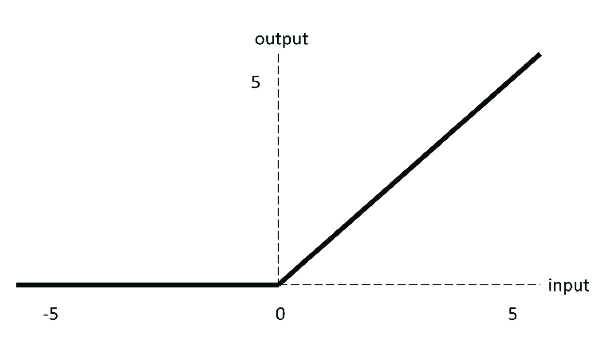
\includegraphics[width=0.7\textwidth]{Procesado de la imagen de color/Classificadores/ReLu.png}
	\caption{Funcionamiento de ReLU(Rectified Linear Unit)}
	\label{fig:ReLu}
	\vspace{-5pt}
\end{figure}


Para reentrenar AlexNet con las nuevas clases es necesario modificarlo ya que este ha sido diseñado para reconocer 1000 clases en lugar de 7. Es necesario eliminar las tres últimas capas que se encargan de la clasificación y sustituirlas por capas similares pero de una correcta dimensión para detectar las siete clases. Los cambios a aplicar son:
\begin{itemize}
\item Capa 23: Fully Connected (1x1x1000) $\rightarrow$ (1x1x7)
\item Capa 24: Softmax (1x1x1000) $\rightarrow$ (1x1x7)
\item Capa 23: Classification output
\end{itemize}

A continuación se muestra la estructura final en la \autoref{fig:LEGONet} y la activación de la primera capa convolucional en la \autoref{fig:LEGONet conv}.
	
\begin{figure}[ht]  %LEGONet
	\centering
	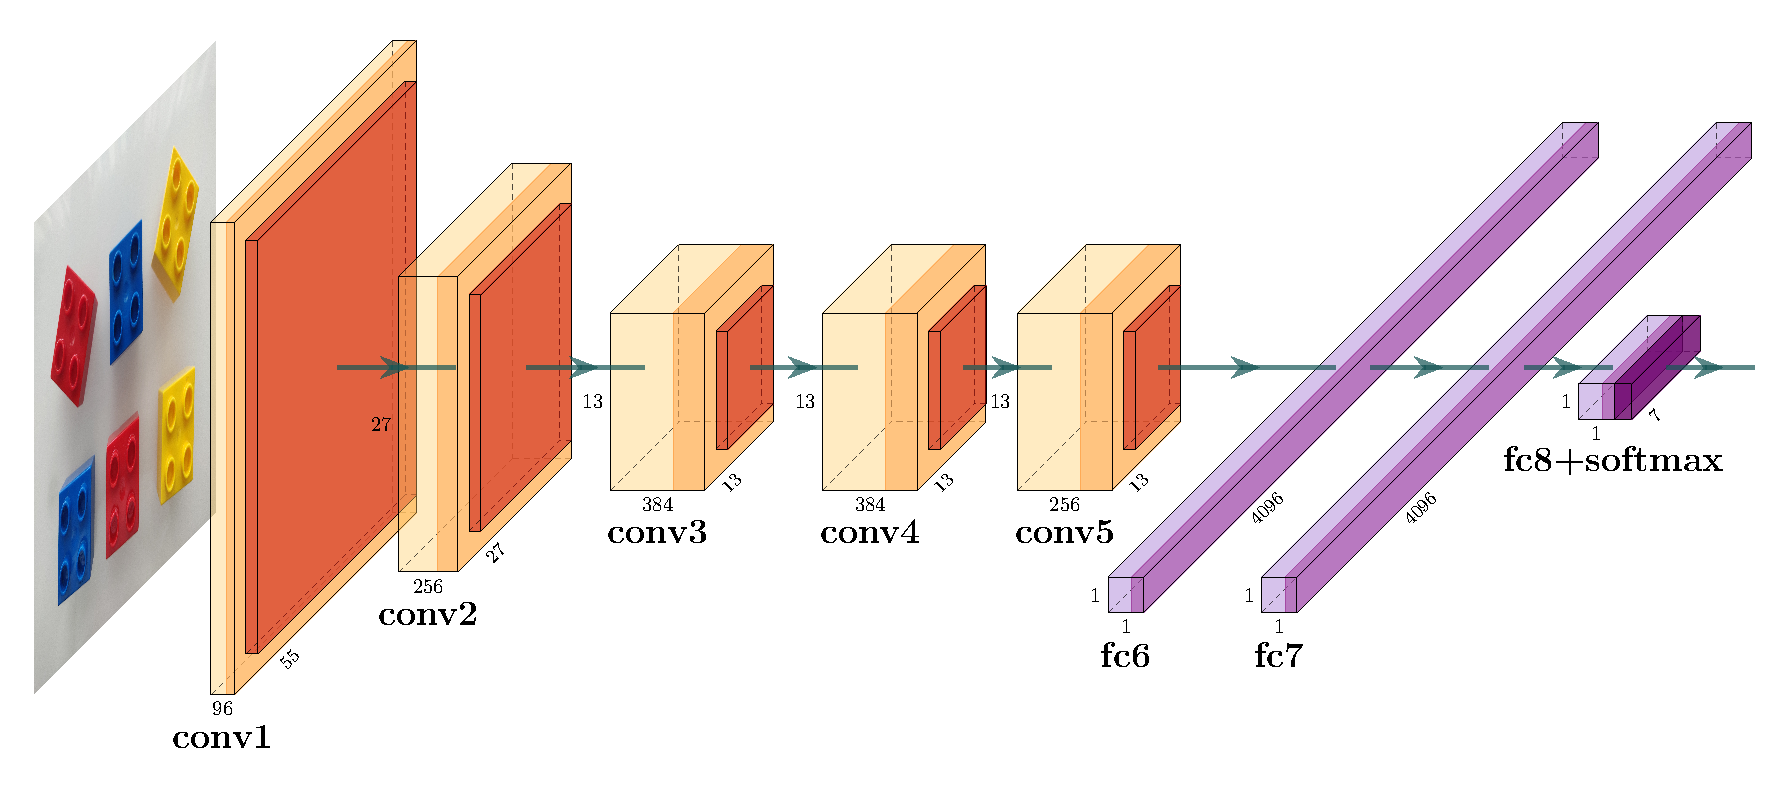
\includegraphics[width=1\textwidth]{Procesado de la imagen de color/Classificadores/LEGONet.pdf}
	\caption{Estructura de LEGONet}
	\label{fig:LEGONet}
	\vspace{-5pt}
\end{figure}

\begin{figure}[ht]  %LEGONet conv
	\centering
	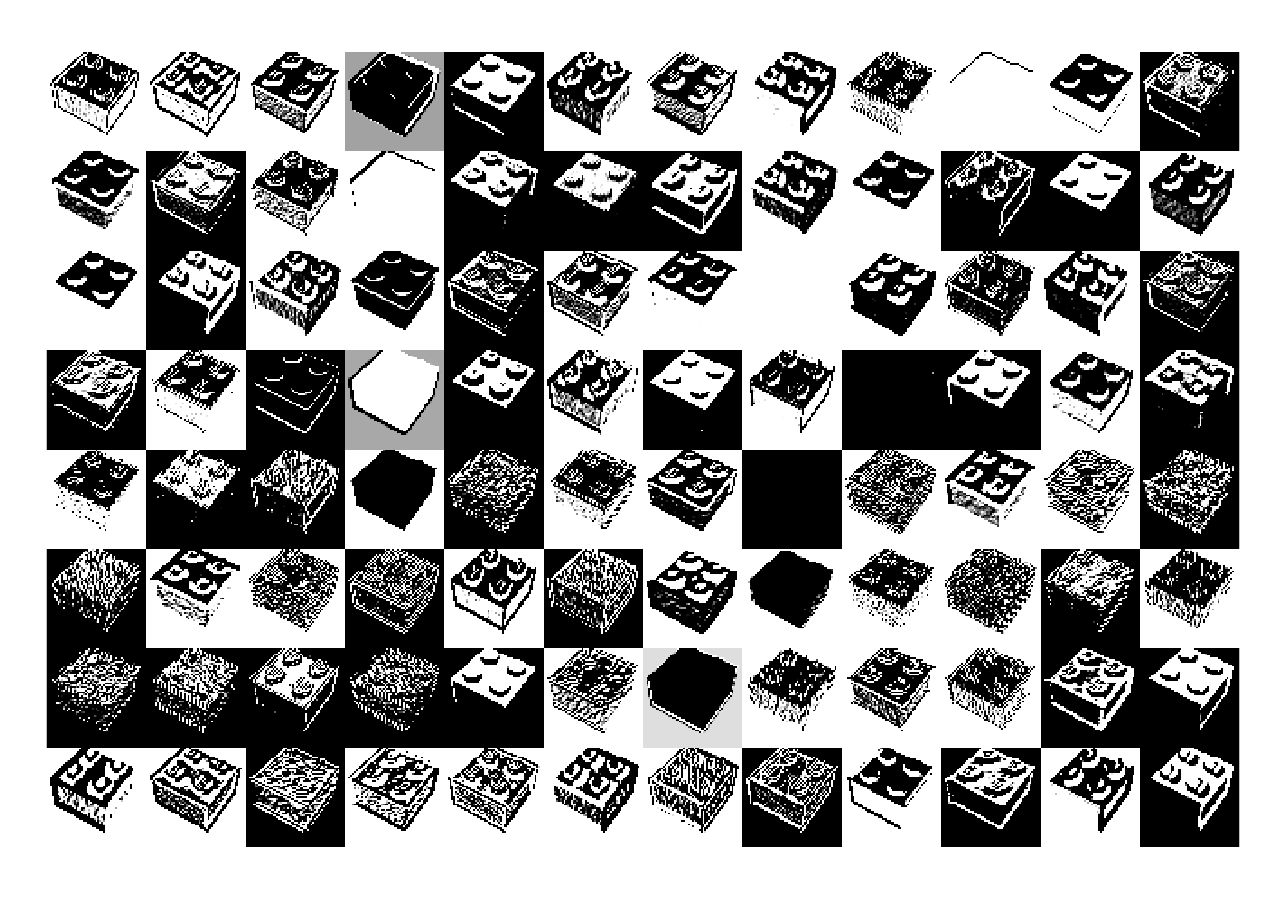
\includegraphics[width=0.8\textwidth]{Procesado de la imagen de color/Classificadores/LEGONet_conv1.png}
	\caption{Activación primera convolución de LEGONet}
	\label{fig:LEGONet conv}
	\vspace{-5pt}
\end{figure}

\subsubsection*{Entrenamiento}
Con la ayuda de MATLAB y del conjunto de imágenes clasificadas por Intel \citep{IntelDataset}, el conjunto de imágenes de LEGOS clasificadas por Joost Hazelzet \citep{LEGODataset} y el conjunto de imágenes de LEGOS clasificadas por Francisco Garcia \citep{LEGODataset2} se ha reentrenado AlexNet para clasificar un total de 7 clases diferentes:

\rev{\begin{itemize}
\item LEGOS: 2464 imágenes
\item Edificios: 2191 imágenes
\item Bosques: 2171 imágenes
\item Glaciares: 2404 imágenes
\item Montañas: 2512 imágenes
\item Calles: 2382 imágenes
\item Océanos: 2274 imágenes
\end{itemize}}

Todo el etrenamiento se ha llevado acabo en un ordenador personal equipado con un i7 4790K, 16GB de memoria RAM y una tarjeta gráfica Nvidia Geforce GTX970 con 4GB de VRAM. Teniendo en cuenta las limitaciones por hardware y tiempo, se han realizado múltiples entrenamiento con diferentes opciones de entrenamiento para obtener los mejores resultados. Tras numerosas pruebas se han seleccionado las siguientes opciones de entrenamiento:

\InsertarCodigo{\Matlab}{images/Procesado de la imagen de color/Classificadores/ClassifierCreation_Alexnet.m}	

\subsubsection*{Resultados}
Con la ayuda de MATLAB y de las bases de datos previamente comentadas, se va a realizar una evaluación del clasificador. En total se han empleado más de 3000 imágenes y a continuación se muestran los resultados obtenidos:

\begin{table}[ht]
  \centering
    \begin{tabular}{|l|r|r|r|r|r|r|r|}
\cline{2-8}    \multicolumn{1}{r|}{} & \multicolumn{1}{l|}{LEGO} & \multicolumn{1}{l|}{Edificio} & \multicolumn{1}{l|}{Bosque} & \multicolumn{1}{l|}{Glaciar} & \multicolumn{1}{l|}{Montaña} & \multicolumn{1}{l|}{Oceano} & \multicolumn{1}{l|}{Calle} \\
    \hline
    LEGO  & 433   & 0     & 0     & 0     & 0     & 1     & 0 \\
    \hline
    Edificio & 0     & 392   & 3     & 0     & 1     & 3     & 35 \\
    \hline
    Bosque & 0     & 0     & 430   & 0     & 3     & 0     & 1 \\
    \hline
    Glaciar & 1     & 1     & 2     & 368   & 42    & 16    & 4 \\
    \hline
    Montaña & 0     & 2     & 0     & 44    & 375   & 12    & 1 \\
    \hline
    Oceano & 2     & 3     & 0     & 6     & 4     & 418   & 1 \\
    \hline
    Calle & 0     & 20    & 0     & 0     & 3     & 0     & 411 \\
    \hline
    \end{tabular}%
  \label{tab:LEGONet results}%
  \caption{Evaluación de LEGONEt: matriz de conteo}
\end{table}%

Analizando estos resultados se puede obtener la tasa de acierto, tasa de fallo y sensibilidad:

\begin{table}[!ht]
  \centering
    \begin{tabular}{|l|r|r|}
\cline{2-3}    \multicolumn{1}{r|}{} & \multicolumn{1}{l|}{Tasa de aciertos} & \multicolumn{1}{l|}{Tasa de fallos} \\
    \hline
    LEGO  & 99,77\% & 0,23\% \\
    \hline
    Edificio & 90,32\% & 9,68\% \\
    \hline
    Bosque & 99,08\% & 0,92\% \\
    \hline
    Glaciar & 84,79\% & 15,21\% \\
    \hline
    Montaña & 86,41\% & 13,59\% \\
    \hline
    Océano & 96,31\% & 3,69\% \\
    \hline
    Calle & 94,70\% & 5,30\% \\
    \hline
    Total & 93,05\% & 6,95\% \\
    \hline
    \end{tabular}%
  \label{tab:LEGONet results2}%
  \caption{Evaluación de LEGONEt: tasa de aciertos y tasa de fallos}
\end{table}%

La tasa de acierto obtenida es bastante elevada si se tiene en cuenta el poco tiempo de entrenamiento y las circunstancias dadas. Si nos fijamos solo el los LEGOS observamos que los resultados son incluso mejores ya que solo ha habido tres falsos positivos y una pieza mal identificada. Es decir, una tasa de acierto al identificar LEGOS del 99.17\%.

\subsection{LEGO16}
En el 2014 VGG-19 y VGG-16 ganaron el primer y segundo puesto de ImageNet y en el 2015 fueron publicadas por Karen Simonyan y Andrew Zisserman en su articulo \textit{"Very Deep Convolutional Networks For Large-Scale Image Recognition"}\cite{VGG16}. Tal y como su nombre indica, estas redes se caracterizan por tener 19 y 16 capas con pesos respectivamente. En este proyecto dadas las limitaciones de hardware y la simplicidad de los objetos a detectar, se ha decantado por el uso de VGG-16 frente a VGG-19.

Para poder emplear VGG-16 ha sido necesario modificarla reemplazando las últimas capas y reentrenarla con varias bases de datos. Esta nueva red se ha nombrado LEGO16.

\subsubsection*{Estructura}
Como su nombre indica, esta red qse caracteriza por tener 16 capas con pesos, un total de 138 millones de parámetros y 13 millones de neuronas . Estas se reparten en 13 capas convolucionales y 3 fully connected. Las capas convolucionales siguen una arquitectura definida donde detrás de cada convolución hay una capa ReLu y asu vez las convoluciones se agrupan en dos grupos de dos y tres grupos de tres. Al final de cada grupo de convoluciones hay una capa Max Pooling para reducir la dimensión. Destaca la inexistencia de las capas Bacth normalization presentes en AlexNet.

Las capas fully connected presentan una arquitectura idéntica a AlexNet por lo que cada capa va acompañada por un capa ReLu y una capa dropout.

Para reentrenar VGG-16 con las nuevas clases es necesario modificarlo ya que este ha sido diseñado para reconocer 1000 clases en lugar de 7. Es necesario eliminar las tres últimas capas que se encargan de la clasificación y sustituirlas por capas similares pero de una correcta dimensión para detectar las siete clases. Los cambios a aplicar son:
\begin{itemize}
\item Capa 23: Fully Connected (1x1x1000) $\rightarrow$ (1x1x7)
\item Capa 24: Softmax (1x1x1000) $\rightarrow$ (1x1x7)
\item Capa 23: Classification output
\end{itemize}

A continuación se muestra la estructura final en la \autoref{fig:LEGO16} y la activación de la primera capa convolucional en la \autoref{fig:LEGO16 conv}.

\begin{figure}[ht]  %LEGO16
	\centering
	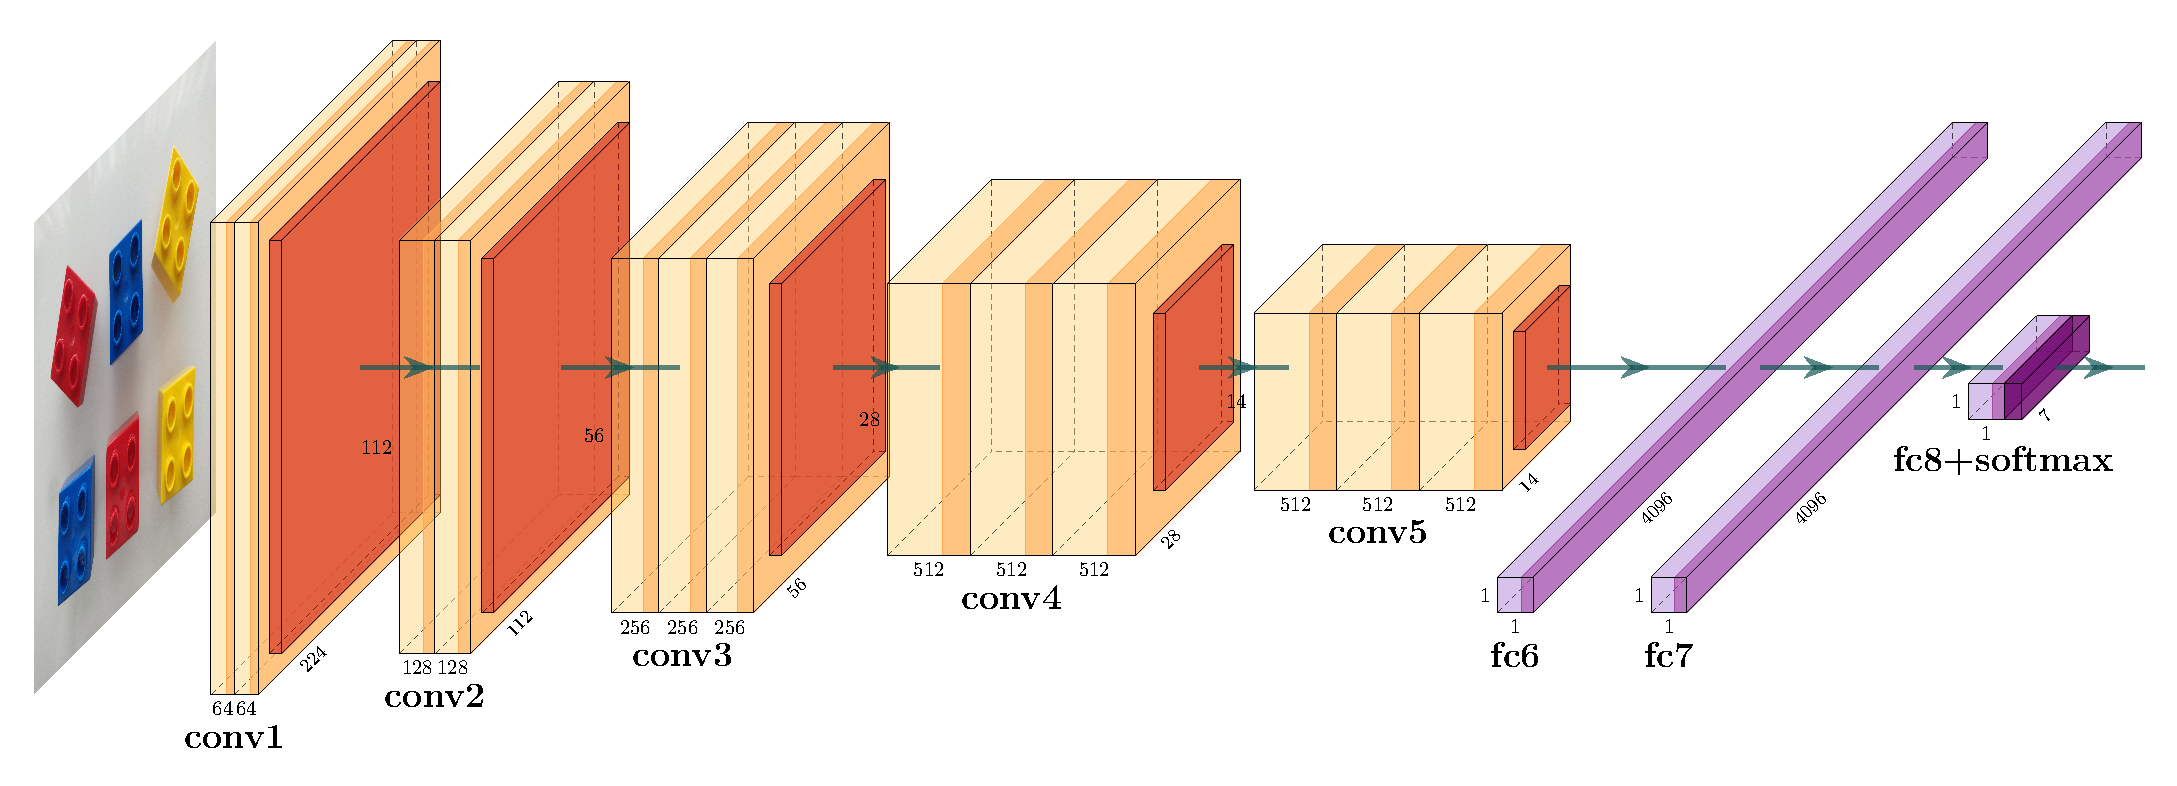
\includegraphics[width=1\textwidth]{Procesado de la imagen de color/Classificadores/LEGO16.pdf}
	\caption{Estructura de LEGO16}
	\label{fig:LEGO16}
	\vspace{-5pt}
\end{figure}

\begin{figure}[ht]  %LEGO16 conv
	\centering
	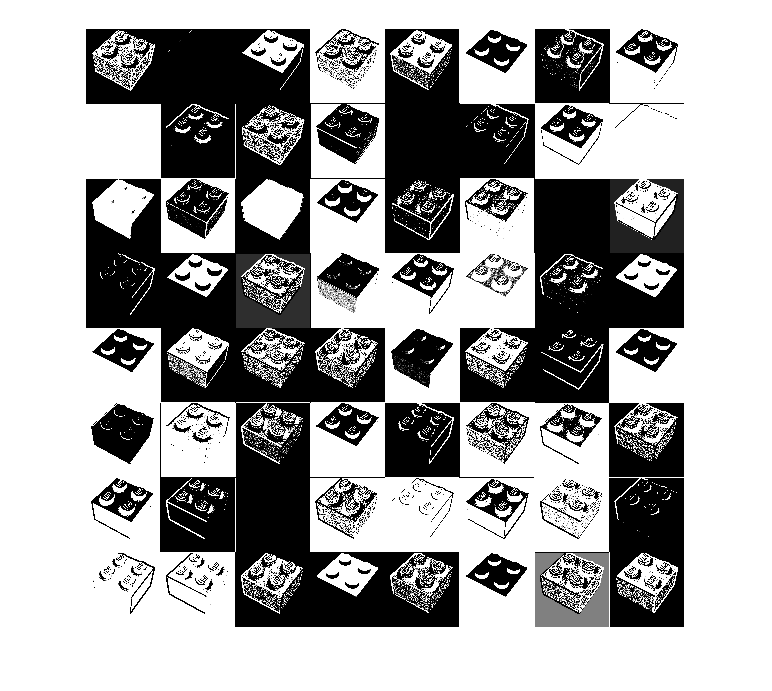
\includegraphics[width=0.8\textwidth]{Procesado de la imagen de color/Classificadores/LEGO16_conv1.png}
	\caption{Activación de la primera convolución de LEGO16}
	\label{fig:LEGO16 conv}
	\vspace{-5pt}
\end{figure}

\subsubsection*{Entrenamiento}
Con la ayuda de MATLAB y del conjunto de imágenes clasificadas por Intel \citep{IntelDataset}, el conjunto de imágenes de LEGOS clasificadas por Joost Hazelzet \citep{LEGODataset} y el conjunto de imágenes de LEGOS clasificadas por Francisco Garcia \citep{LEGODataset2} se ha reentrenado AlexNet para clasificar un total de 7 clases diferentes:

\begin{itemize}
\item LEGOS: 2464 imágenes
\item Edificios: 2191 imágenes
\item Bosques: 2171 imágenes
\item Glaciares: 2404 imágenes
\item Montañas: 2512 imágenes
\item Calles: 2382 imágenes
\item Océanos: 2274 imágenes
\end{itemize}

Todo el etrenamiento se ha llevado acabo en un ordenador personal equipado con un i7 4790K, 16GB de memoria RAM y una tarjeta gráfica Nvidia Geforce GTX970 con 4GB de VRAM. Teniendo en cuenta las limitaciones por hardware y tiempo, se han realizado múltiples entrenamiento con diferentes opciones de entrenamiento para obtener los mejores resultados. Tras numerosas pruebas se han seleccionado las siguientes opciones de entrenamiento:

\InsertarCodigo{\Matlab}{images/Procesado de la imagen de color/Classificadores/ClassifierCreation_VGG16.m}

\subsubsection*{Resultados}
Con la ayuda de MATLAB y de las bases de datos previamente comentadas, se va a realizar una evaluación del clasificador. En total se han empleado más de 3000 imágenes y a continuación se muestran los resultados obtenidos:

\begin{table}[ht]
  \centering
    \begin{tabular}{|l|*{7}{r|}}
\cline{2-8}    \multicolumn{1}{r|}{} & \multicolumn{1}{l|}{LEGO} & \multicolumn{1}{l|}{Edificio} & \multicolumn{1}{l|}{Bosque} & \multicolumn{1}{l|}{Glaciar} & \multicolumn{1}{l|}{Montaña} & \multicolumn{1}{l|}{Oceano} & \multicolumn{1}{l|}{Calle} \\
    \hline
    LEGO  & 433   & 0     & 0     & 0     & 0     & 1     & 0 \\
    \hline
    Edificio & 0     & 401   & 1     & 0     & 0     & 2     & 30 \\
    \hline
    Bosque & 0     & 0     & 432   & 1     & 1     & 0     & 0 \\
    \hline
    Glaciar & 0     & 2     & 1     & 379   & 41    & 9    & 2 \\
    \hline
    Montaña & 0     & 0     & 0     & 34    & 393   & 6    & 1 \\
    \hline
    Oceano & 1     & 1     & 1     & 4     & 2     & 425   & 0 \\
    \hline
    Calle & 0     & 19    & 1     & 0     & 0     & 2     & 412 \\
    \hline
    \end{tabular}%
  \label{tab:LEGO16 results}%
  \caption{Evaluación de LEGO16: matriz de conteo}
\end{table}%

Analizando estos resultados se puede obtener la tasa de acierto, tasa de fallo y sensibilidad:

\begin{table}[htbp]
  \centering
  \caption{Add caption}
    \begin{tabular}{|l|r|r|}
\cline{2-3}    \multicolumn{1}{r|}{} & \multicolumn{1}{l|}{Tasa de aciertos} & \multicolumn{1}{l|}{Tasa de fallos} \\
    \hline
    LEGO  & 99,77\% & 0,23\% \\
    \hline
    Edificio & 92,40\% & 7,60\% \\
    \hline
    Bosque & 99,54\% & 0,46\% \\
    \hline
    Glaciar & 87,33\% & 12,67\% \\
    \hline
    Montaña & 90,55\% & 9,45\% \\
    \hline
    Océano & 97,93\% & 2,07\% \\
    \hline
    Calle & 94,93\% & 5,07\% \\
    \hline
    Total & 94,63\% & 5,37\% \\
    \hline
    \end{tabular}%
  \label{tab:LEGO16 results2}%
  \caption{Evaluación de LEGO16: tasa de aciertos y tasa de fallos}
\end{table}%

La tasa de acierto obtenida es bastante elevada si se tiene en cuenta el poco tiempo de entrenamiento y las circunstancias dadas. Si nos fijamos solo el los LEGOS observamos que los resultados son incluso mejores ya que solo ha habido tres falsos positivos y una pieza mal identificada. Es decir, una tasa de acierto al identificar LEGOS del 99.17\%.

En general, este clasificador ha dado mejores resultados frente a LEGONet a pesar de contar con las limitaciones de hardware. Probablemente se puedan obtener mejores resultados si se consigue entrenar durante más tiempo a la red y con más datos. Además, es conveniente emplear hardware más potente para poder entrenar con un mayor número de imágenes a la vez. De esta forma se pueden evitar problemas por regularización.

\section{RCNN}
\label{sec:RCNN}
